\documentclass{article}
\usepackage[utf8]{inputenc}
\usepackage{graphicx}
\usepackage{amsmath}
\usepackage{booktabs}
\usepackage{textcomp}
\usepackage{multirow}
\usepackage{color}
\usepackage{listings}

\lstset{
	numbers=left,
	basicstyle=\small,
	tabsize=3,
	showspaces=false,
	showtabs=false,
	showstringspaces=false
}
\title{Assignment 1.5}
\author{Christian M\"uller, Ralph Krimmel \& Sebastian Albert }

\begin{document}
\maketitle
\section*{(a)}
The disk service time $T_S$  is defined as the sum of the seek time, the rotational latency and the data transfer time. \\
\begin{equation}
T_S = \text{seek time} + \text{rotational latency} + \text{data transfer time}
\end{equation}
The summands of this equation will be explained in detail now.
\subsection*{Seek time}
Refering to the lecture slides, the seek time is the time to position the read/write head and is specified by the manufacturer.
\subsection*{Rotational latency}
According to the lecture slides, the rotational latency is the time taken by the plater to rotate and position the data under the read/write head and is dependent on the rotation speed of the spindle. The formula to calculate the rotational latency for a given rotation speed $X$ is \\
\begin{equation}
\text{Rotational latency} = \frac{0.5}{\frac{X}{60}}
\end{equation}
\subsection*{Data transfer time}
The lecture slides define the data transfer time/rate as the average amount of data per unit time that the drive can deliver to the Host bus adaptor. This value is, like the seek time,  also specified by the manufacturer.

\section*{(b)}
The maximum IOPS that a disk can service depends upon the disk service time $T_S$. 
\begin{eqnarray*}
T_S &=& \text{Seek time} + \frac{0.5}{(\frac{\text{Disk rpm}}{60})} + \frac{\text{Data block size}}{\text{Data transfer rate}} \\
    &=& 5ms + \frac{0.5}{(\frac{7200rpm}{60})} + \frac{64KB}{\frac{40MB}{s}}\\
    &=& 5ms + 4.1ms + 1.6ms \\
    &=& 10.7ms
\end{eqnarray*}

The maximum IOPS can be calculated by computing $\frac{1sec}{T_S}$ = 93 IOPS.

\section*{(c)}
The average response time of a controller depends on its utilization. For acceptable response times, the utilization of the disk controller must be less than 70\% of its maximum. Therefore, to calculate the actual IOPS that a disk can service, its maximum IOPS has to be multiplied by 0.7.

\section*{(d)}
The average response time R can be calculated with the following equation:
\begin{equation}
R = \frac{T_S}{(1-U)}
\end{equation}
where U is the utilization of the disk controller. Figure \ref{fig:responsetime} shows the average response time over changing utilizatipn levels. We can see that the response time increases at 70\% utilization up to levels where a proper operation is no longer possible. Therefore, a the disk should not be utilized over 70\% of its capacity.

\begin{figure}
	\begin{center}
	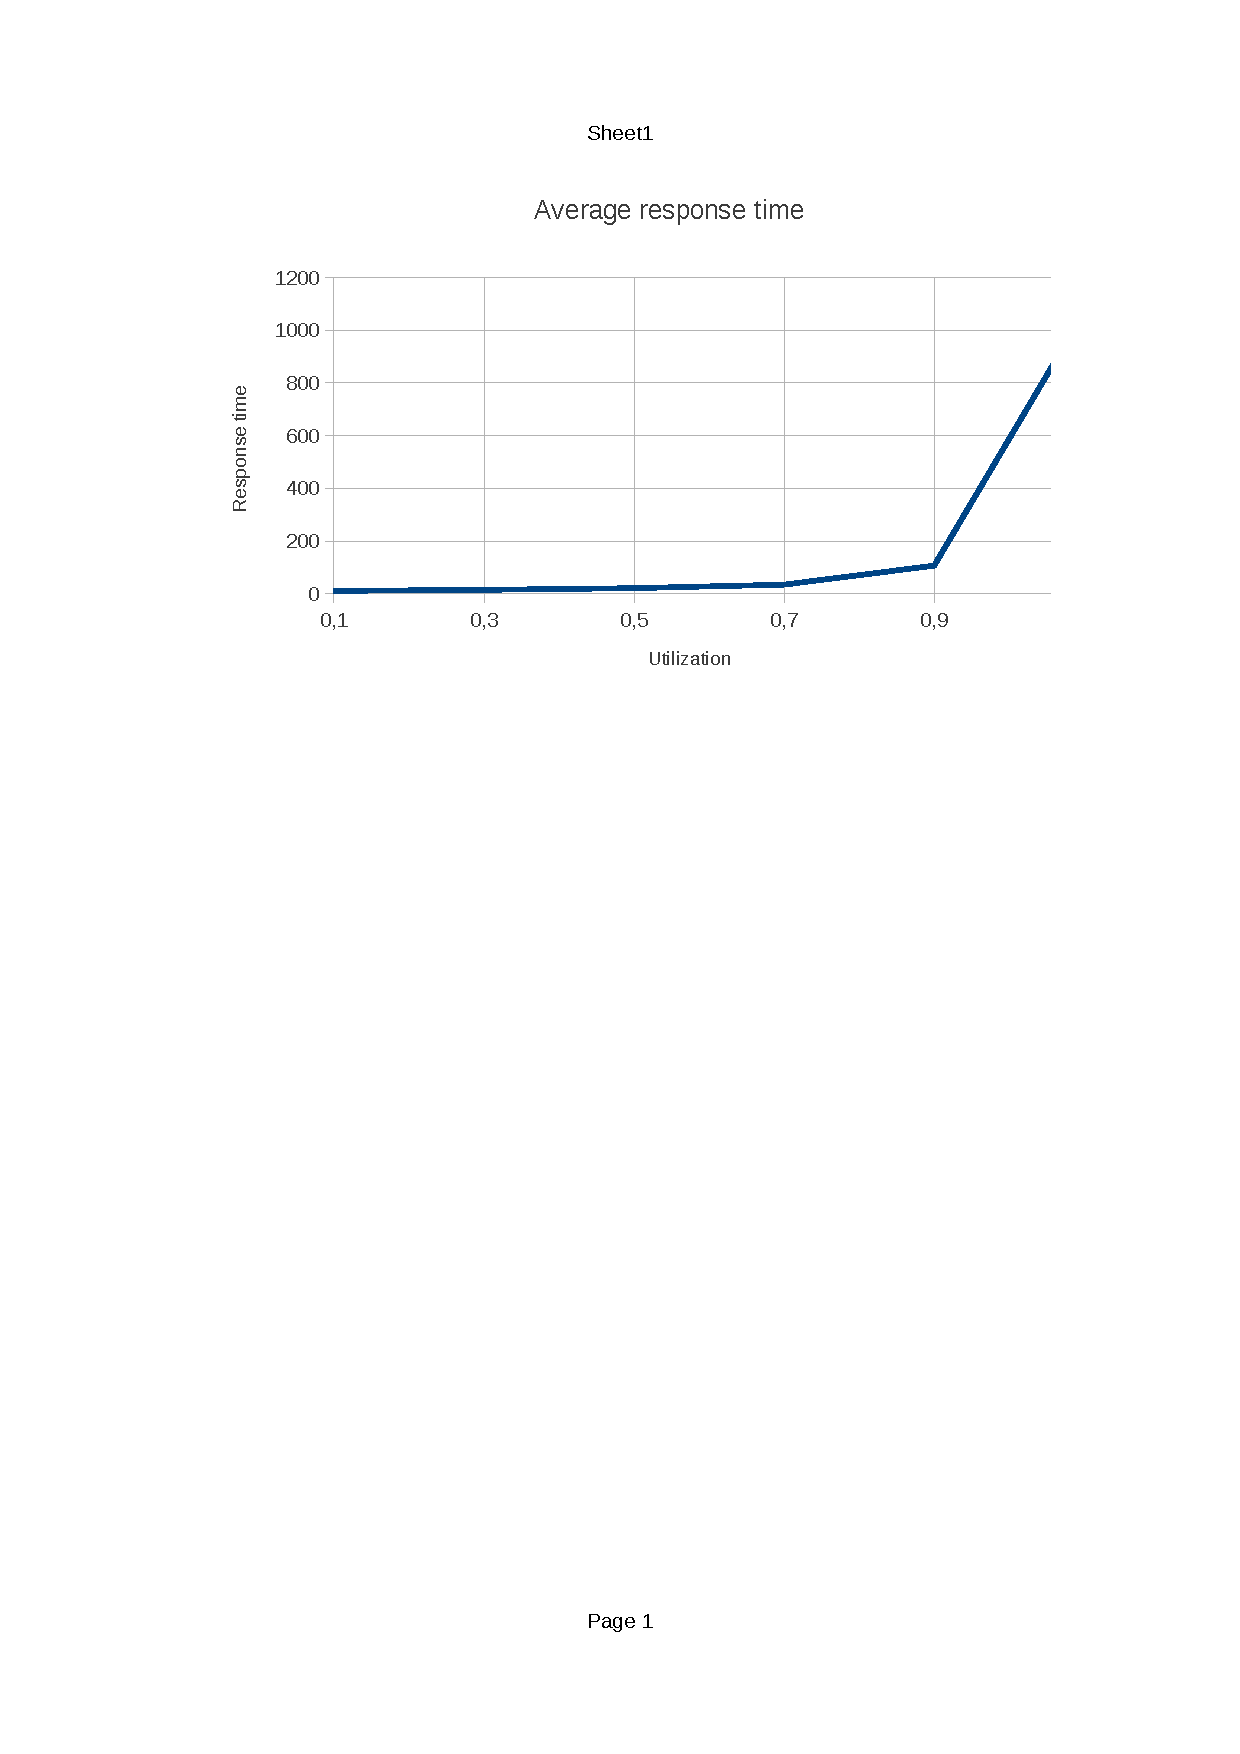
\includegraphics[width=\textwidth]{plot.pdf}
	\caption{Average response times over changing utilization levels of the hard disk}
	\label{fig:responsetime}
	\end{center}
\end{figure}



\section*{(e)}
Formatted partitions contain a filesystem, which itself needs additional space for meta or other data (e.g. Journals, checkpoints) to be operatable. Also some filesystems reserve space that just can be acceses as administrator in case of a full harddisk.

\end{document}
